% !TEX TS-program = xelatex
% !TEX encoding = UTF-8 Unicode 

% \documentclass[AutoFakeBold]{LZUThesis}
\documentclass[AutoFakeBold]{LZUThesis}
\usepackage{multirow}
\usepackage{threeparttable}
\CTEXsetup[name={第,部分}]{chapter}
\lstset{
language = MATLAB,
backgroundcolor=\color{white},   % choose the background color; you must add \usepackage{color} or \usepackage{xcolor}  
basicstyle=\footnotesize,        % the size of the fonts that are used for the code  
breakatwhitespace=false,         % sets if automatic breaks should only happen at whitespace  
breaklines=true,                 % sets automatic line breaking  
captionpos=bl,                    % sets the caption-position to bottom  
% commentstyle=\color{green},    % comment style  
% deletekeywords={...},            % if you want to delete keywords from the given language  
% escapeinside={\%*}{*)},          % if you want to add LaTeX within your code  
extendedchars=true,              % lets you use non-ASCII characters; for 8-bits encodings only, does not work with UTF-8  
frame=shadowbox,                    % adds a frame around the code  
keepspaces=true,                 % keeps spaces in text, useful for keeping indentation of code (possibly needs columns=flexible)  
keywordstyle=\color{blue},       % keyword style  
% language=Python,                 % the language of the code  
morekeywords={*,...},            % if you want to add more keywords to the set  
numbers=left,                    % where to put the line-numbers; possible values are (none, left, right)  
numbersep=5pt,                   % how far the line-numbers are from the code  
numberstyle=\tiny\color{gray}, % the style that is used for the line-numbers  
rulecolor=\color{black},         % if not set, the frame-color may be changed on line-breaks within not-black text (e.g. comments (green here))  
showspaces=false,                % show spaces everywhere adding particular underscores; it overrides 'showstringspaces'  
showstringspaces=false,          % underline spaces within strings only  
showtabs=false,                  % show tabs within strings adding particular underscores  
stepnumber=1,                    % the step between two line-numbers. If it's 1, each line will be numbered  
stringstyle=\color{orange},     % string literal style  
tabsize=2,                       % sets default tabsize to 2 spaces  
% title=signalAnalysis.m           % show the filename of files included with \lstinputlisting; also try caption instead of title  
}  

\begin{document}
%=====%
%
%封皮页填写内容
%
%=====%

% 标题样式 使用 \title{{}}; 使用时必须保证至少两个外侧括号
%  如: 短标题 \title{{第一行}},  
% 	      长标题 \title{{第一行}{第二行}}
%             超长标题\tiitle{{第一行}{...}{第N行}}

\title{{反馈放大器设计的自我理解}}



% 标题样式 使用 \entitle{{}}; 使用时必须保证至少两个外侧括号
%  如: 短标题 \entitle{{First row}},  
% 	      长标题 \entitle{{First row}{ Second row}}
%             超长标题\entitle{{First row}{...}{ Next N row}}
% 注意:  英文标题多行时 需要在开头加个空格 防止摘要标题处英语单词粘连.

\author{\CJKfontspec{楷体}李文涛}
\major{电子信息基地班}
\college{320200928101}
\grade{2020级}



\maketitle
\frontmatter

%中文摘要
\ZhAbstract{
该篇反馈放大器设计向我展现了指定频段下的放大器设计过程,通过设计电阻电容反馈回路,调整放大器的频率响应并优化响应过程,使其在直流(或者说低频段)能够按照指定的要求进行反馈放大。在设计过程中,还考虑了外界环境(如温度)对系统的影响,引入了“增益灵敏度”的概念,辅证了负反馈在实际使用中的稳定性。整个设计令我更好地理解了课上所学的波特图在实际系统中所呈现的作用。在这篇论文里,我叙述我对反馈放大器的设计过程的理解。
}{负反馈、波特图、设计}




%生成目录
% \tableofcontents
% \addcontentsline{toc}{chapter}{目录}
% \thispagestyle{empty}


%文章主体
\mainmatter

\chapter{设计过程}

\section{明确目标}
文章提出了设计要求——直流增益为10的放大器,但实际情况是源信号中会掺杂其他频段的信号,文章中首先建立了运算放大器的开环传递函数:

\begin{equation}
a(s)=\frac{a_0}{(1+s/\omega_1)(1+s/\omega_2)}
\end{equation}

其中的$a(s)$、$\omega_1$、$\omega_2$都为较大的值,显然在实际使用中我们需要对这个系统添加反馈环节进行调整。为了将问题进行解决。文章中将该开环传递函数的频率响应做出以便进行下一布的设计。

在这次设计中,首先我们对放大器的增益和调整时间的要求下进行了设计和更改,然后又针对更改后所出现的调整过程的多次震荡建立电路,补偿其相位裕量。

\section{调整增益大小及调整时间}
通过引入电阻分压电路来进行负反馈,达到改变增益大小和调整时间的目的,负反馈能够有效地加快系统的瞬态响应,反馈电路以及数学描述如下所示:

\begin{figure}[htbp]
    \centering
    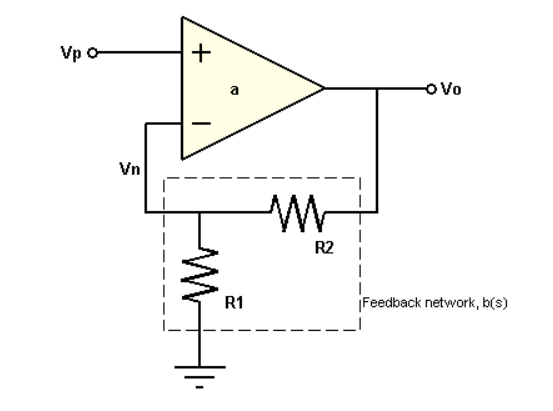
\includegraphics[keepaspectratio,width=300pt]{1.png}
    \caption{反馈电路模型图}
\end{figure}

\begin{figure}[htbp]
    \centering
    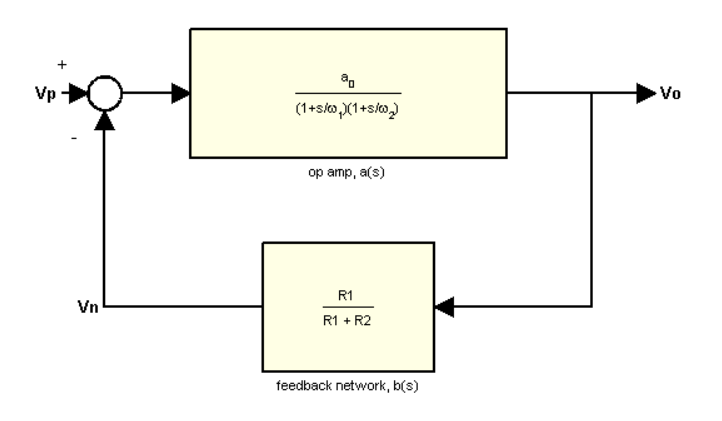
\includegraphics[keepaspectratio,width=400pt]{2.png}
    \caption{反馈电路数学描述}
\end{figure}

在这一步设计中,我们将开环传递部分定为$a(s)$,反馈部分定为$b(s)$以便进行下一步的分析处理。通过分压的关系,我们很容易得出$b(s)$的传递函数:

\begin{equation}
    b=V_n / V_o = R1 / (R1 + R2)
\end{equation}

同时写出总的闭环增益为:

\begin{equation}
    A = Vo / Vp = A / (1 + ab)
\end{equation}

如果乘积ab足够大(>>1),则A(s)可以近似为$A=1/b$,所以我们可以通过固定其中一个电阻来通过我们要求的增益大小来确定另一个电阻的大小:

\begin{equation}
    \begin{aligned}
    A0 &= 10  \\
    R1 &= 10000 \\
    R2 &= R1 * (1/b - 1)=90000
    \end{aligned}
\end{equation}

将我们当前设计的反馈电路作频率相应图进行分析,观察开环增益和闭环增益的区别。
\begin{figure}[htbp]
    \centering
    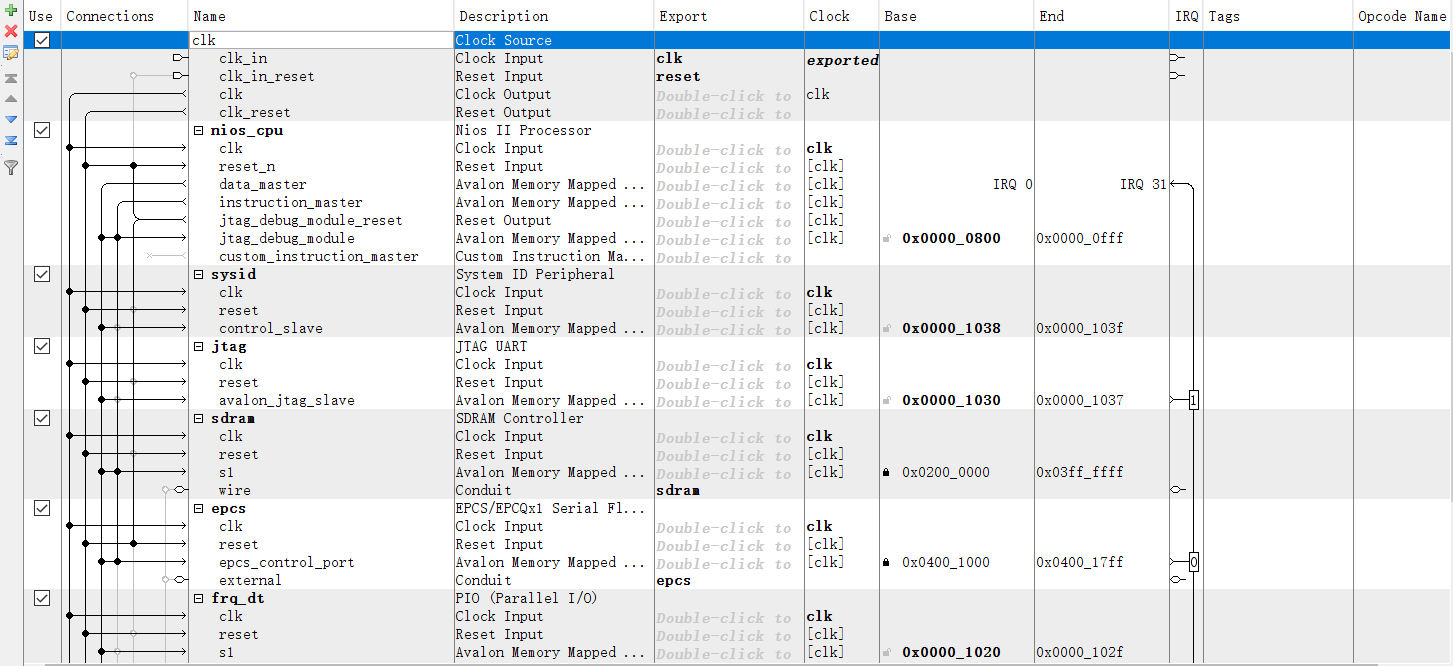
\includegraphics[keepaspectratio,width=400pt]{3.png}
    \caption{系统开环增益与闭环增益波特图}
\end{figure}
我们知道,反馈能减小参数变化以及干扰对系统输出的影响,这里我们从另外一个角度说明负反馈的好处。由于增益现在由反馈网络控制,因此要考虑的一个有用关系是该增益对运放自然(开环)增益变化的灵敏度,这里称其为“系统灵敏度”。

在推导系统灵敏度之前,我们首先定义一下环路增益$L(s)=a(s)b(s)$,它是信号在环路上传播的总增益。这便于我们对系统的灵敏度和稳定性作进一步分析。

我们写出系统灵敏度的表达式:
\begin{equation}
    S=\frac{\delta A/A}{\delta a/a}=\frac{1}{1+a(s)b(s)}=\frac{1}{1+L(s)}
\end{equation}

而后文章指出“$S(s)$与反馈方程具有相同的形式,因此可以使用更鲁棒的FEEDBACK命令来构造
”,随即我们做出两者的波特图(增益幅度)进行分析:

\begin{figure}[htbp]
    \centering
    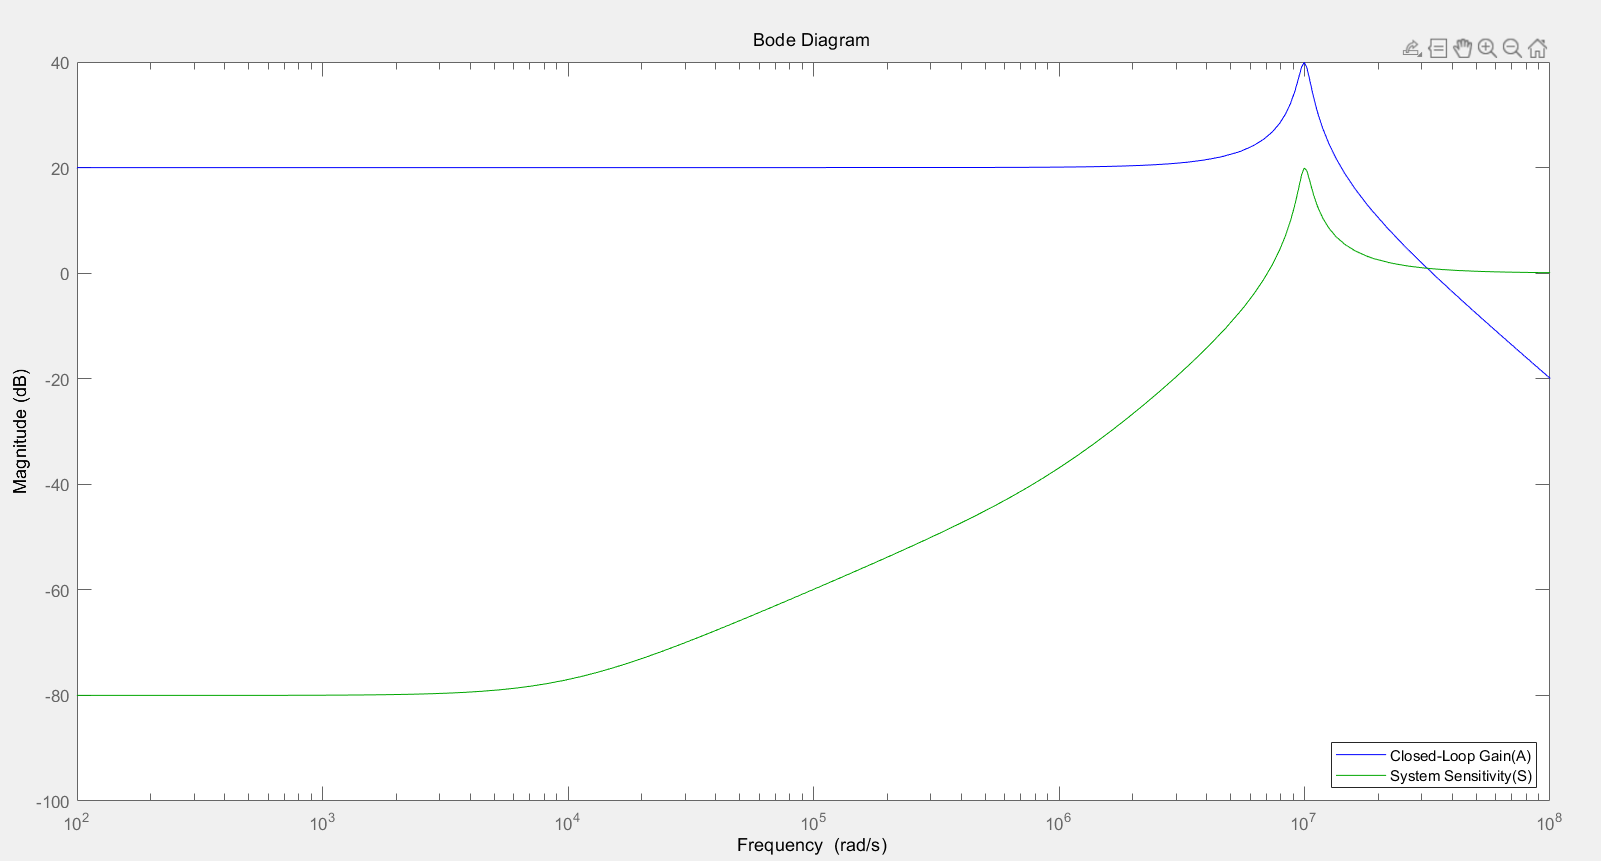
\includegraphics[keepaspectratio,width=400pt]{4.png}
    \caption{系统A(s)与S(s)的增益波特图}
\end{figure}

我们观察到在低频时系统具有非常小的灵敏度(约- 80db),表明此时该设计的闭环增益受开环增益变化的影响最小。在实际系统的生产使用过程中,由于制造变化、温度变化等原因,A(s)会发生变化,此时我们的低频灵敏度低便更能说明系统的稳定性。

\section{补偿相位裕量}
我们检查系统的阶跃响应发现,其稳定时间大大降低,但是在稳定之前发生了多次的震荡,这显然不是我们所愿意看到的。

\begin{figure}[htbp]
    \centering
    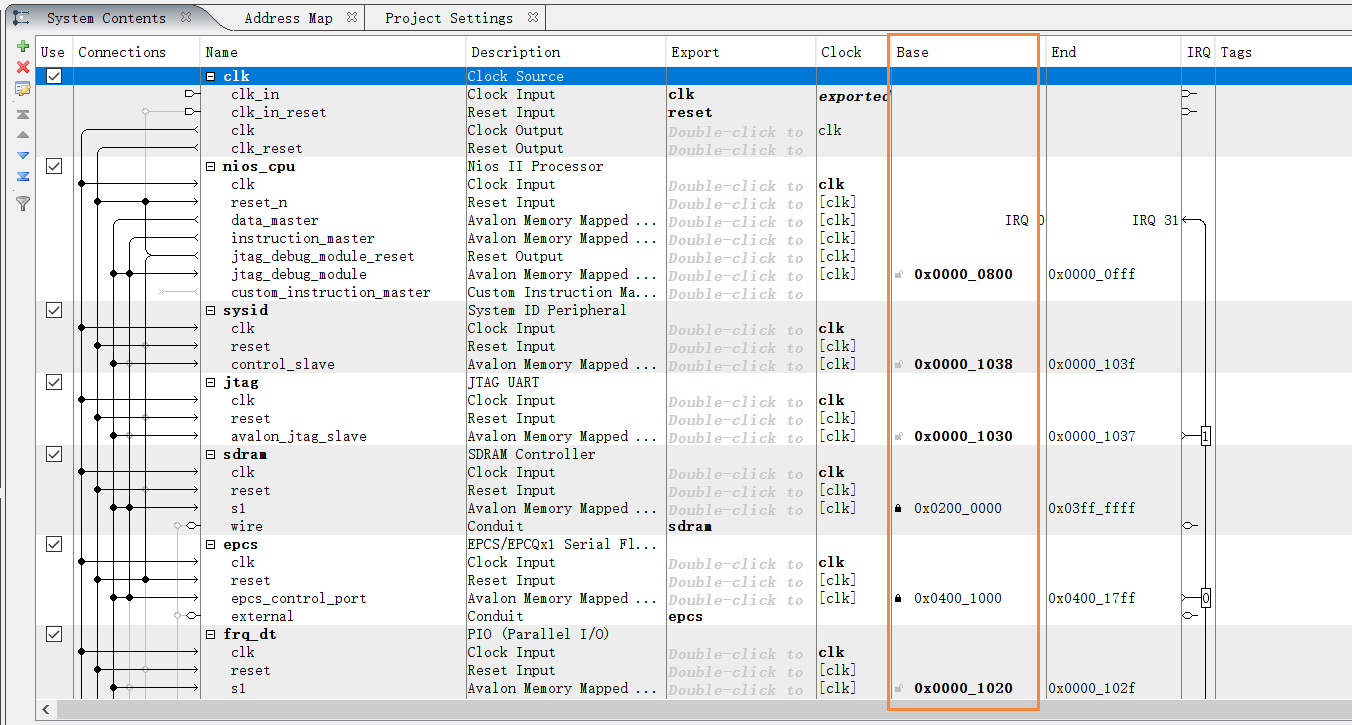
\includegraphics[keepaspectratio,width=400pt]{5.png}
    \caption{系统的阶跃响应}
\end{figure}

我们利用margin命令绘制回路增益L(s)来分析其相对稳定性(即增益裕量和相位裕量)。

\begin{figure}[htbp]
    \centering
    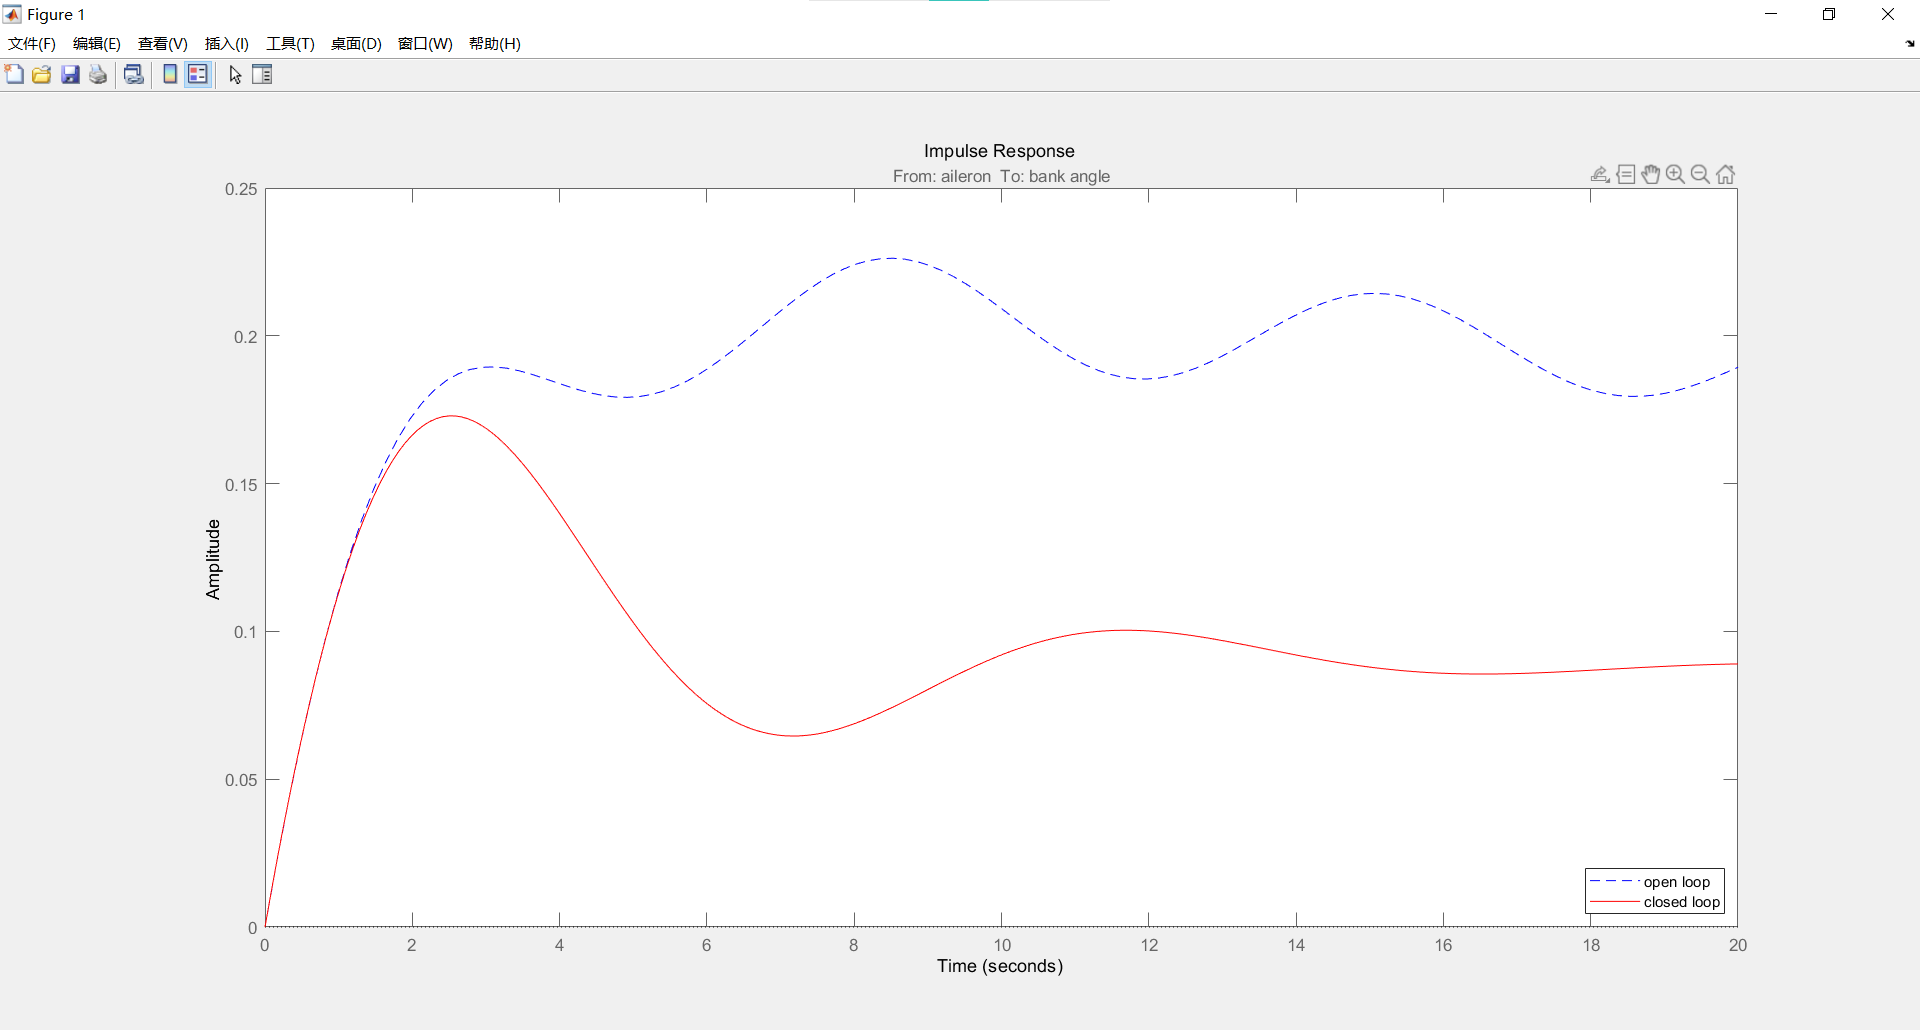
\includegraphics[keepaspectratio,width=400pt]{6.png}
    \caption{L(s)的波特图}
\end{figure}

图中明显显示相位裕量为$180-174=6$度,在课上我们知道,在工程上我们要求这个数值一般在30到60之间,现在显然不符合要求。
这里就是这篇文章给我带来的最大收获,它提出了一种补偿方式即feedback lead compensation,
通过在反馈电阻R2并联上添加电容C来修改b(s)。
选择电容器值以便在交叉频率附近向b(s)引入一个超前相位,从而增加放大器的相位裕度。
引入电容后的反馈电路的示意图如下:
\begin{figure}[htbp]
    \centering
    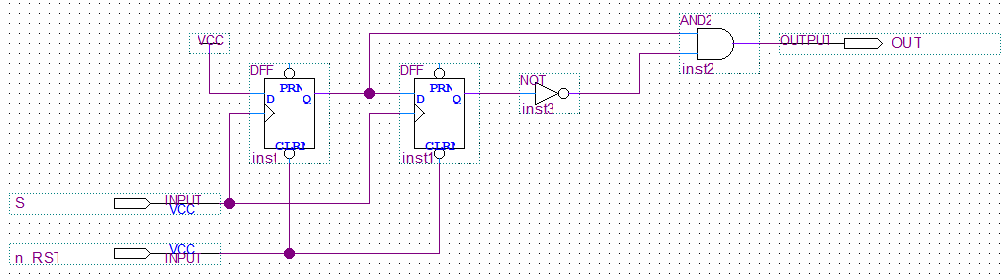
\includegraphics[keepaspectratio,width=300pt]{8.png}
    \caption{新反馈电路模型图}
\end{figure}

\begin{figure}[htbp]
    \centering
    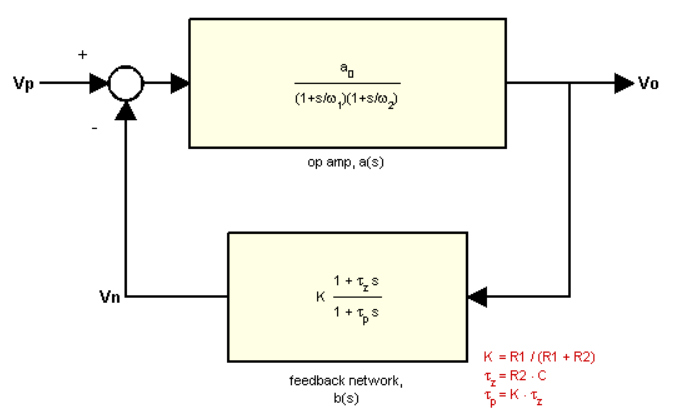
\includegraphics[keepaspectratio,width=300pt]{7.png}
    \caption{新反馈电路数学描述}
\end{figure}

接下来来确定C的值,我们可以通过剪切频率来近似C的值$(C = 1/(R2*W_{cp}))$。
当然,为了更为精确地得到电容值的大小,我们可以利用matlab的计算能力为A(s)和L(s)建立LTI数组,类似于遍历将随着C的大小变化的系统阶跃响应一一绘制出来,进而观察电容值的变化对系统稳定性的影响。

\begin{figure}[htbp]
    \centering
    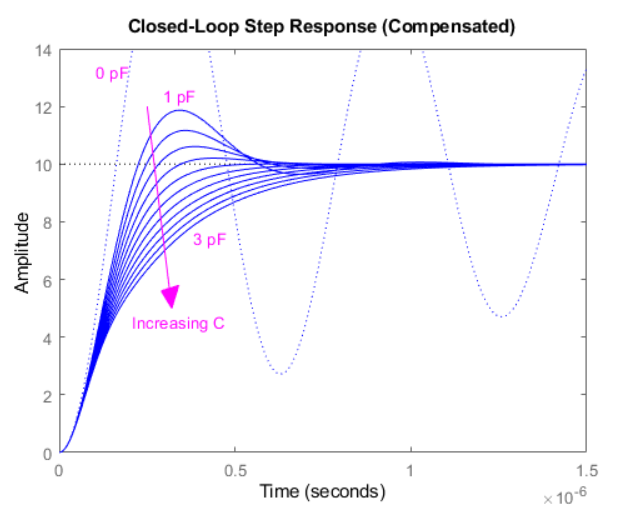
\includegraphics[keepaspectratio,width=300pt]{9.png}
    \caption{不同电容值下系统的阶跃响应}
\end{figure}

进一步得出各个C下系统的相位裕量,这样我们就可以将C与相位裕量通过函数联系在一起,从而选择出最优解。作出相位裕量随着C变化的函数关系图如下


\begin{figure}[htbp]
    \centering
    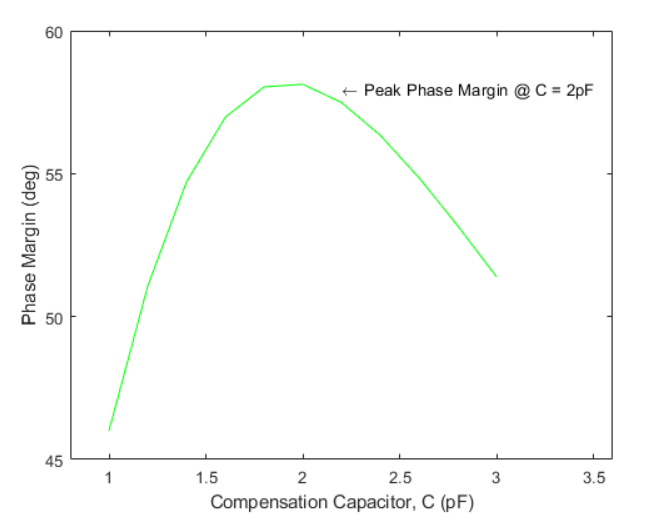
\includegraphics[keepaspectratio,width=300pt]{10.png}
    \caption{相位裕量随着C变化的函数关系}
\end{figure}

得到当C=2pF时,可获得58度的最大相位裕度。故我们选择电容值为2pF,并做出加上电容器前后系统的阶跃响应进行对比:

\begin{figure}[htbp]
    \centering
    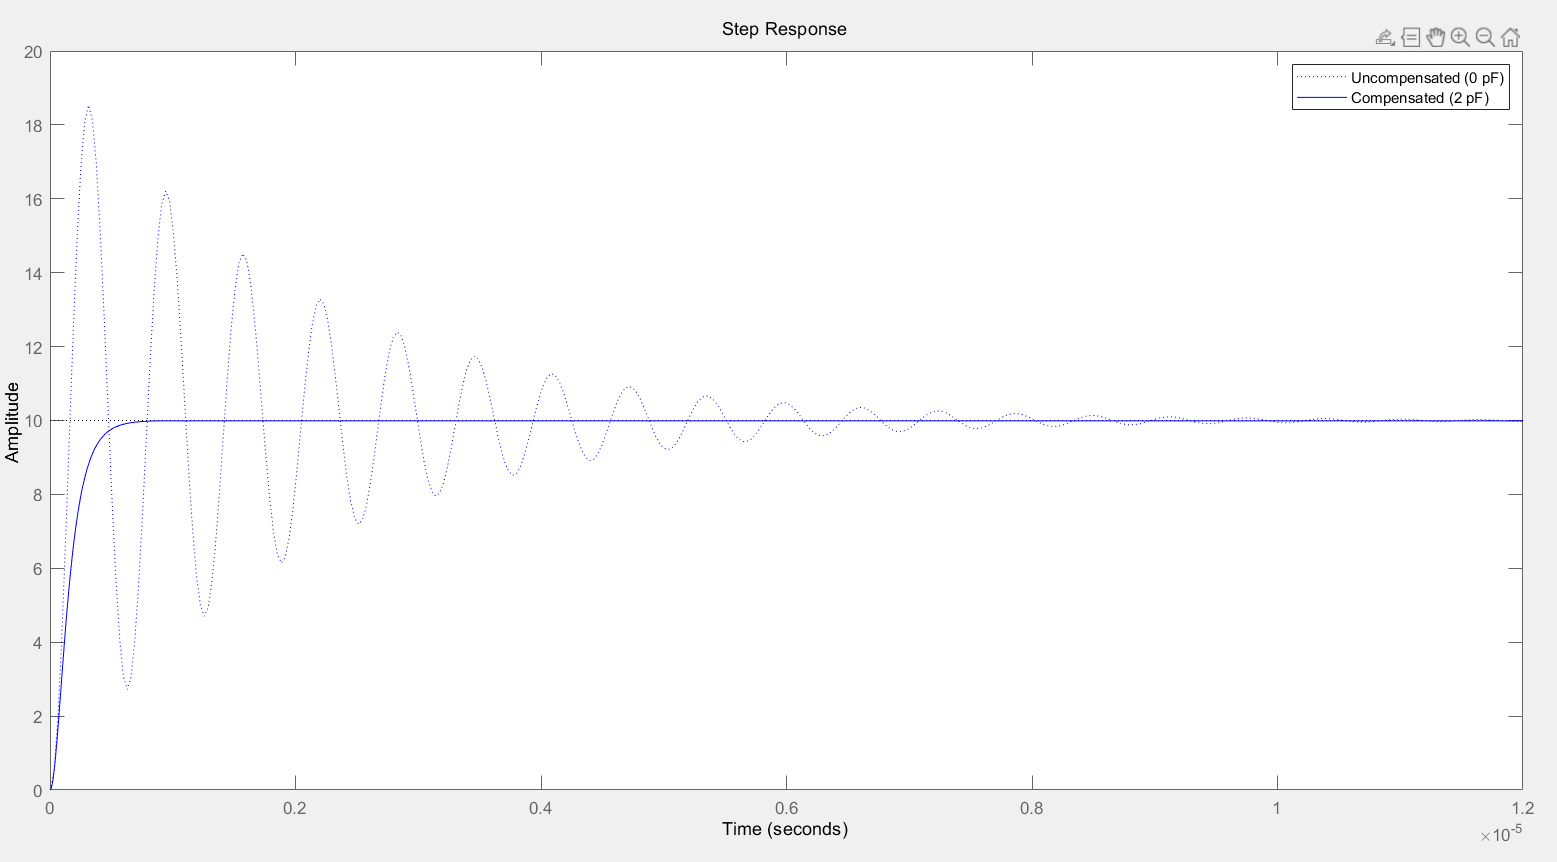
\includegraphics[keepaspectratio,width=300pt]{11.png}
    \caption{增添电容前后系统的阶跃响应}
\end{figure}

稳定性明显得到改善。

\chapter{探究收获}
通过理解这种非反相反馈放大器电路设计,我对自动控制系统的设计有了更深一步的了解,最大的收获是如何通过利用波特图分析系统的增益裕量和相位裕量来控制系统的相对稳定性。

在这次设计中,我们最终选择了电阻反馈网络来产生10(20dB)的放大器,并选择了2pF的电容来扩大系统的相位裕量来保证系统的相对稳定性。

在课上学习到的各个知识点在设计过程中都有着很好的对应,使我的自动控制原理有了现实应用的照应,帮助我更好地理解自动控制原理的模型构建与分析。在实际设计中还要考虑反馈时的实际情况,根据实际情况来调整对反馈系统的要求,就如这次设计中的“系统灵敏度”。






\backmatter


% %=======%
% %引入参考文献文件
% %=======%
\bibdatabase{bib/POC}%bib文件名称 仅修改bib/ 后部分
\printbib
\nocite{*} %显示数据库中有的,但是正文没有引用的文献


% \Appendix

% 这里是附录页,可要可不要

% \Thanks.



\end{document}